% !TeX program = XeLaTeX
\documentclass[cs4size,sub3section,UTF8,nofonts,SlantFont,fancyhdr,hyperref,fntef]{ctexart}\usepackage[]{graphicx}\usepackage[]{color}
%% maxwidth is the original width if it is less than linewidth
%% otherwise use linewidth (to make sure the graphics do not exceed the margin)
\makeatletter
\def\maxwidth{ %
  \ifdim\Gin@nat@width>\linewidth
    \linewidth
  \else
    \Gin@nat@width
  \fi
}
\makeatother

\definecolor{fgcolor}{rgb}{0.345, 0.345, 0.345}
\newcommand{\hlnum}[1]{\textcolor[rgb]{0.686,0.059,0.569}{#1}}%
\newcommand{\hlstr}[1]{\textcolor[rgb]{0.192,0.494,0.8}{#1}}%
\newcommand{\hlcom}[1]{\textcolor[rgb]{0.678,0.584,0.686}{\textit{#1}}}%
\newcommand{\hlopt}[1]{\textcolor[rgb]{0,0,0}{#1}}%
\newcommand{\hlstd}[1]{\textcolor[rgb]{0.345,0.345,0.345}{#1}}%
\newcommand{\hlkwa}[1]{\textcolor[rgb]{0.161,0.373,0.58}{\textbf{#1}}}%
\newcommand{\hlkwb}[1]{\textcolor[rgb]{0.69,0.353,0.396}{#1}}%
\newcommand{\hlkwc}[1]{\textcolor[rgb]{0.333,0.667,0.333}{#1}}%
\newcommand{\hlkwd}[1]{\textcolor[rgb]{0.737,0.353,0.396}{\textbf{#1}}}%

\usepackage{framed}
\makeatletter
\newenvironment{kframe}{%
 \def\at@end@of@kframe{}%
 \ifinner\ifhmode%
  \def\at@end@of@kframe{\end{minipage}}%
  \begin{minipage}{\columnwidth}%
 \fi\fi%
 \def\FrameCommand##1{\hskip\@totalleftmargin \hskip-\fboxsep
 \colorbox{shadecolor}{##1}\hskip-\fboxsep
     % There is no \\@totalrightmargin, so:
     \hskip-\linewidth \hskip-\@totalleftmargin \hskip\columnwidth}%
 \MakeFramed {\advance\hsize-\width
   \@totalleftmargin\z@ \linewidth\hsize
   \@setminipage}}%
 {\par\unskip\endMakeFramed%
 \at@end@of@kframe}
\makeatother

\definecolor{shadecolor}{rgb}{.97, .97, .97}
\definecolor{messagecolor}{rgb}{0, 0, 0}
\definecolor{warningcolor}{rgb}{1, 0, 1}
\definecolor{errorcolor}{rgb}{1, 0, 0}
\newenvironment{knitrout}{}{} % an empty environment to be redefined in TeX

\usepackage{alltt}
\usepackage{amsmath}
\usepackage{amsfonts}
\usepackage{amssymb}
\usepackage{siunitx}
\usepackage{textcomp}
\usepackage{graphicx}
\usepackage[includeheadfoot,top=3.5cm,bottom=3.0cm,left=3.5cm,right=3.0cm]{geometry}
\author{Yang Ling}
\title{CTeX}

\pagestyle{fancy}
\renewcommand{\headrule}{\hrule width\textwidth}	%页眉线填满文本宽度
\rhead{}
\fancyhead[C]{\zihao{5}浙江大学\LaTeX 测试}	%页眉

\usepackage{xunicode,xltxtra}
\defaultfontfeatures{Mapping=tex-text}

\setCJKmainfont{H-秀月}
\setCJKsansfont[BoldFont={* Bold}]{微软雅黑}
\setCJKmonofont{H-宫书}
\newCJKfontfamily[yalan]\yalan{H-新雅兰}
\newCJKfontfamily[HSS]\HSS{H-SS}
%\newCJKfontfamily[apple]\apple[BoldFont={* W6}]{Hiragino Sans GB}

%\setmainfont{Times New Roman}
\setsansfont{League Script Thin}

\CTEXsetup[format={\Large\bfseries}]{section}
\CTEXsetup[format+={\CJKunderdot}]{section}
\CTEXsetup[name={第,章}]{section}
\CTEXsetup[number={\chinese{section}}]{section}

\CTEXoptions[today=big]

\usepackage[unicode=true,xetex,pdfstartview=FitH,bookmarks=true,bookmarksnumbered=true,bookmarksopen=true,colorlinks=true,pdfborder=001,citecolor=magenta,linkcolor=blue]{hyperref}	%hyperref 宏包通常要求放在导言区的最后!!!
\hypersetup{pdfauthor={Yang Ling,China Zhejiang University,<kaji331@hotmail.com>}}	%pdf文档属性.
\IfFileExists{upquote.sty}{\usepackage{upquote}}{}

\begin{document}

\CTEXnumber{\money}{2012}
\section{\CTeX~\XeLaTeX 测试}
\zihao{-3}\today zju欠了我\money 圆整!\tt\num{1d7}, \numlist{10;20;30;40}, \numrange{10}{100}, \si{\milli\liter, \degreeCelsius}, \textcelsius, \texteuro

\tt\textsl{静}\textbf{夜}\textit{思}
\begin{center}
静夜思\\
床前明月光,疑似地上霜。\\
举头望明月,低头思故乡。
\end{center}

\yalan\textbf{夜登白帝城怀少陵先生}
\begin{center}
夜登白帝城怀少陵先生\\
拾遗白发有谁怜?零落歌诗遍两川。\\
人立飞楼今已矣,浪翻孤月尚依然。\\
升沈自古无穷事,愚智同归有限年。\\
此意凄凉谁共语?岸沙君看去年痕。
\end{center}

\sf\textbf{桃源行}
\begin{center}
《桃源行》\\
To be or not to be\\
作者:王维\\
渔舟逐水爱山春,两岸桃花夹去津。\\
坐看红树不知远,行尽青溪忽视人。\\
山口潜行始隈隩,山开旷望旋平陆。\\
遥看一处攒云树,近入千家散花竹。\\
樵客初传汉姓名,居人未改秦衣服。\\
居人共住武陵源,还从物外起田园。\\
月明松下房栊静,日出云中鸡犬喧。\\
惊闻俗客争来集,竞引还家问都邑。\\
平明闾巷扫花开,薄暮渔樵乘水入。\\
初因避地去人间,及至成仙遂不还。\\
峡里谁知有人事,世中遥望空云山。\\
不疑灵境难闻见,尘心未尽思乡县。\\
出洞无论隔山水,辞家终拟长游衍。\\
自谓经过旧不迷,安知峰壑今来变。\\
当时只记入山深,青溪几曲到云林。\\
春来遍是桃花水,不辨仙源何处寻。
\end{center}

\rm
\begin{center}
《审判异性恋》\\
『没那么简单』\\
作者:难勃丸/一瓶果酱\\
怎能不悲哀,一直以来,没有人来爱。\\
摆正心态,告诉自己一人也精彩。\\
满是尘埃,不懂去爱,我的心长满了青苔。\\
怎能不悲哀,徒有黑白,还有啥期待。\\
独自感慨,心已枯单身才最自在。\\
沧海桑田,心不摇摆,抱歉已不耐烦未来。\\
对于生活已失去动力,对于爱情也毅然放弃。\\
若然心不动,也就不会痛,道理谁都懂。\\
满街喧哗拥挤人潮里,一堆一堆的情侣。\\
团友在召集,带上打火机,代表月亮惩罚你。\\
异性恋由我来审判,天下情侣通通拆散。\\
求赦免没那么简单,秀恩爱将牢底坐穿。\\
孤独一万年单身汉,寂寞在每一个夜晚。\\
烧死这一大群异端,至少分我个,可以分我个,好汉。
\end{center}

\HSS
\begin{center}
高端大气上档次,\\
低调奢华有内涵,\\
简约时尚国际范,\\
奔放洋气有深度,\\
低端粗俗甩节操,\\
土鳖矫情无下限,\\
装模作样绿茶婊,\\
外猛内柔女汉子,\\
卖萌嘟嘴剪刀手,\\
忧郁深沉无所谓,\\
狂拽帅气叼炸天,\\
冷艳高贵接地气,\\
时尚亮丽小清新,\\
可爱乡村非主流,\\
贵族王朝杀马特,\\
提莫团战必须死。
\end{center}

\begin{kframe}
\begin{alltt}
\hlkwd{library}\hlstd{(xtable)}
\hlstd{c} \hlkwb{<-} \hlkwd{xtable}\hlstd{(}\hlkwd{summary}\hlstd{(cars))}
\hlkwd{print}\hlstd{(c,} \hlkwc{type} \hlstd{=} \hlstr{"latex"}\hlstd{)}
\end{alltt}
\end{kframe}% latex table generated in R 3.0.2 by xtable 1.7-1 package
% Tue Dec 31 22:08:37 2013
\begin{table}[ht]
\centering
\begin{tabular}{rll}
  \hline
 &     speed &      dist \\ 
  \hline
1 & Min.   : 4.0   & Min.   :  2   \\ 
  2 & 1st Qu.:12.0   & 1st Qu.: 26   \\ 
  3 & Median :15.0   & Median : 36   \\ 
  4 & Mean   :15.4   & Mean   : 43   \\ 
  5 & 3rd Qu.:19.0   & 3rd Qu.: 56   \\ 
  6 & Max.   :25.0   & Max.   :120   \\ 
   \hline
\end{tabular}
\end{table}
\begin{kframe}\begin{alltt}
\hlkwd{plot}\hlstd{(cars)}
\end{alltt}
\end{kframe}
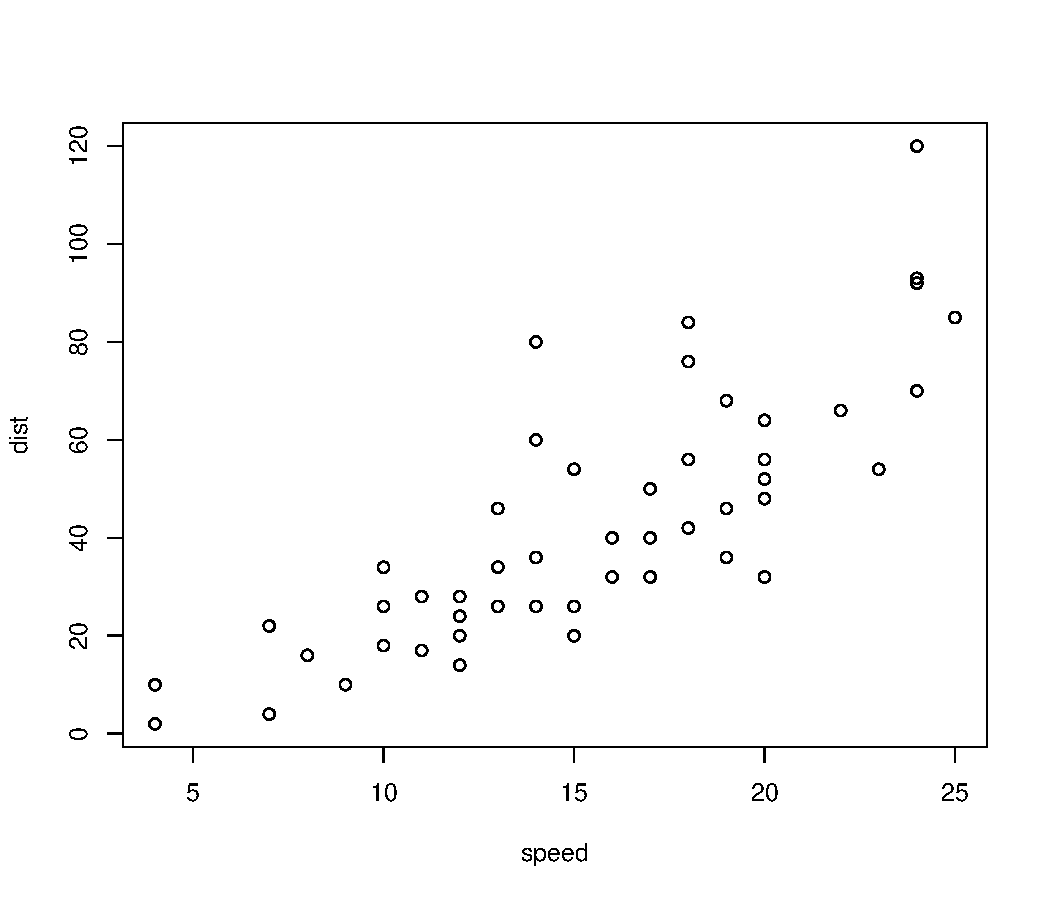
\includegraphics[width=\maxwidth]{figure/example} 



\centering
$\Gamma = \beta_0 + {\beta_1}^2 + \sum_{n=1}^{10}$

\end{document}
